\documentclass{article}

% if you need to pass options to natbib, use, e.g.:
% \PassOptionsToPackage{numbers, compress}{natbib}
% before loading nips_2016
%
% to avoid loading the natbib package, add option nonatbib:
% \usepackage[nonatbib]{nips_2016}

% \usepackage{nips_2016}

% to compile a camera-ready version, add the [final] option, e.g.:
\usepackage[final]{proposal}

\usepackage[utf8]{inputenc} % allow utf-8 input
\usepackage[T1]{fontenc}    % use 8-bit T1 fonts
\usepackage{hyperref}       % hyperlinks
\usepackage{url}            % simple URL typesetting
\usepackage{booktabs}       % professional-quality tables
\usepackage{amsfonts}       % blackboard math symbols
\usepackage{nicefrac}       % compact symbols for 1/2, etc.
\usepackage{microtype}      % microtypography
\usepackage{graphicx}
\title{A Reinforcement Learning based HVAC Control for Thermal Comfort and Energy Efficiency \\in Office Buildings
}

% The \author macro works with any number of authors. There are two
% commands used to separate the names and addresses of multiple
% authors: \And and \AND.
%
% Using \And between authors leaves it to LaTeX to determine where to
% break the lines. Using \AND forces a line break at that point. So,
% if LaTeX puts 3 of 4 authors names on the first line, and the last
% on the second line, try using \AND instead of \And before the third
% author name.

\author{
  Zhiang Zhang\\
  \And 
  Siliang Lu\\
  \And 
  Chenlu Zhang\\
  %% examples of more authors
  %% \And
  %% Coauthor \\
  %% Affiliation \\
  %% Address \\
  %% \texttt{email} \\
  %% \AND
  %% Coauthor \\
  %% Affiliation \\
  %% Address \\
  %% \texttt{email} \\
  %% \And
  %% Coauthor \\
  %% Affiliation \\
  %% Address \\
  %% \texttt{email} \\
  %% \And
  %% Coauthor \\
  %% Affiliation \\
  %% Address \\
  %% \texttt{email} \\
}


\begin{document}
% \nipsfinalcopy is no longer used

\maketitle


\section{Introduction}
\subsection{...}
The application of reinforcement learning to building HVAC control is not yet well explored in building research. Liu and Henze [5, 6] implemented a Q-learning algorithm with Neural Network as the Q function approximation method to control the global building temperature setpoint and active thermal storage charge/discharge rate. The objective is to reduce the HVAC operation cost during the cooling season. Through a simulation study based on one level of a building, it was found that reinforcement learning can achieve 22\% cost saving compared to the conventional rule-based control. However, the authors mentioned that the learning period for the reinforcement learning is too long to be realistic for the real-life application. A similar application of reinforcement learning was reported in [7], where authors use fitted Q iteration method to find the optimal action for the heater's on/off. The objective is also cost saving of HVAC operation. The algorithm was tested in a simulation model of a room, and it was found after 20 days of learning, the algorithm can reach 90\% of the performance of a MPC algorithm (viewed as the "true" optimal solution). Dalamagkidis [8] implemented a linear reinforcement learning controller (using linear functions to approximate the value function) based on TD learning algorithm to control the heat pump, air ventilation system and window opening. The authors found the reinforcement learning controller can only achieve similar energy efficiency and thermal comfort performance with the conventional controllers, but takes significant time to learn. It can be found that there is no agreement on the performance of the reinforcement learning controller in the HVAC systems. In this project, the team plans to build the work based on the above mentioned researches, and try to evaluate the feasibility of the reinforcement learning control for the building HVAC systems. 

\subsection{...}
...

  
 %The heat balance theory and physiology of human thermo-regulatory system identify that occupant's thermal comfort is affected by both indoor environment conditions  and occupant conditions . Therefore, to provide a comfortable indoor environment, the control algorithm of the HVAC system should deal with building thermal behavior, weather.  
 
 %Since  and dynamic, occupants sitting at different location of the office will experience different thermal environment. However, most offices can only be controlled at zone level, rather than individual level. 
 
 %The concept of thermal adaptation shows that, in addition to instant environment surrounding occupants, thermal comfort is also affected by occupant's past thermal experience and expectation, as well as other context-dependent factors, such as age, gender, and weight.[3] Even two occupant sharing same thermal environment may have distinct thermal sensation.  In conclusion, the  challenges in improving thermal comfort of a group of occupants in a shared office are the non-uniform thermal environment, the discrepancy of occupants, and the disturbances to the environment. 
 
  

\section{Methods}

\section{Preliminary Results}
\subsection{Simulator}
EnergyPlus is used as the simulator for the building and its HVAC system simulation. It is developed by the U.S. Department of Energy and is widely used by researchers and engineers for building performance evaluation and optimization[ref????]. 

To use the EnergyPlus simulator more conveniently, we developed a simulator extending the OpenAI gym interface and wrapping the EnergyPlus simulation engine inside. The schematic diagram of the implementation is shown in the Figure \ref{fig:eplus_env}.  
\begin{figure}[h]
\centering
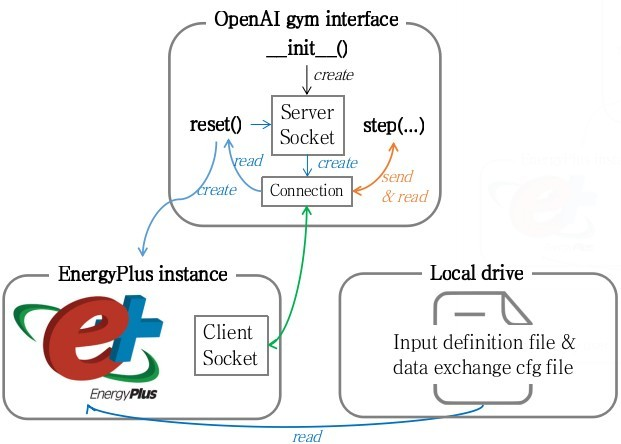
\includegraphics[width=0.8\textwidth]{eplus_env.jpg}
\caption{EnergyPlus environment in OpenAI gym}
\label{fig:eplus_env}
\end{figure} 

EnergyPlus is a standalone program. Therefore, to integrate it into the OpenAI gym environment, we used the socket communication to exchange the information between EnergyPlus program and the \textit{OpenAI gym environment}. During the OpenAI gym environment \textit{initialization}, it creates a Socket as the \textit{server socket}. When \textit{reset} is called, the gym environment firstly initiates an new \textit{EnergyPlus instance}. This EnergyPlus instance reads its \textit{input definition file} (IDF) and \textit{data exchange configuration file} (CFG) from the \textit{local drive} to determine the building model information and data exchange information (will be explained later). The EnergyPlus program also automatically creates a \textit{client socket} to connect with the server in the OpenAI gym environment. The OpenAI gym environment will then capture the \textit{connection} with EnergyPlus's client socket. Then, the server will read the first observation from the EnergyPlus instance. When \textit{step} is called, the server in the OpenAI gym environment sends the actions to the EnergyPlus instance and reads the observation and other information from the EnergyPlus instance through the connection between the server and the client. After one episode ends, the \textit{EnergyPlus instance} and the \textit{connection} will be discarded. 

EnergyPlus is just a simulation engine. The building model is defined by the IDF file, which includes the building geometry, thermal properties, HVAC system topology, system properties, etc. The building model used for this project is a one-story 5-zone office building. It is assumed the building is located in Pittsburgh, PA, USA. The HAVC system is the centralized variable air volume system with terminal reheat. The building has one air handling unit serving all five zones, and the primary heating/cooling source is DX-coil. Simulation time step is 900 seconds, and running period for one episode is Jan 1st 00:00:00 to Mar 31st 24:00:00. 

For this project, only one zone of the building model is used for reinforcement learning and control, even though the building model has five zones. The selected zone is located on the south part of the building, with area 99.16 m2, lighting load 16.1 W/m2, equipment load 10.8 W/m2, maximum occupant number 11. The occupancy density in the zone has regular office work pattern. The zone has a single air conditioning air outlet. The supply air flow rate of the outlet can be controlled independently, but the supply air temperature is subject to the supply air temperature from the centralized HVAC system because the zone has only a terminal heating coil, no cooling coil.

$loss = -\delta log(\pi(A|S, \theta)) $

\section{Final Plan}

\section*{References}

\end{document}

